\section{Métodos da Posição Falsa e da Posição Falsa Modificado}
%\index{Métodos da Posição Falsa e da Posição Falsa Modificado}

\subsection{Método da Posição Falsa}

\begin{enumerate}
 \item Esse método difere do método da bisseção apenas na forma como o ponto \underline{b} é calculado.

\begin{figure}[htb]
  %\index{figura da posição falsa}%
  \setlength{\abovecaptionskip}{20pt}
  %%% o valor default de \abovecaptionskip definido para a classe
  %%% article e de 10pt.
  \centering
  %%% VIDE ABAIXO COMENTARIO SOBRE USO DE DIRETORIOS NO PATHNAME
  %%% DOS ARQUIVOS INCLUIDOS.
  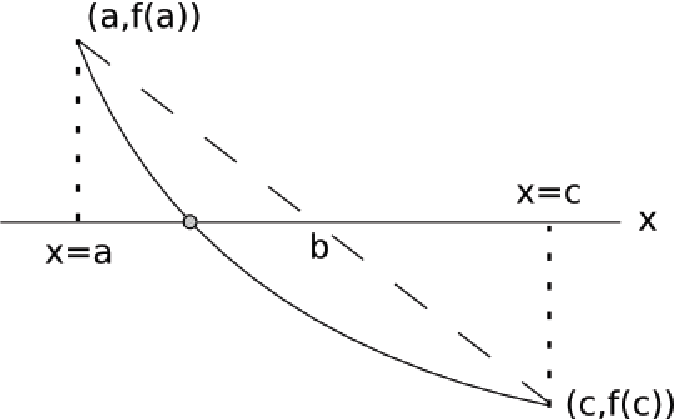
\includegraphics[scale=0.8]{capitulos/capitulo1/figuras/posicaofalsa1-eps-converted-to.pdf}
  \caption{Método da Posição Falsa}
  \label{fig:posicaofalsa1}
\end{figure}

\begin{equation}
 \label{eq:posicaofalsa1}
 y = f(a) + \frac{f(c) - f(a)}{c - a} \ast (x - a)
\end{equation}

Para $y = 0$ na equação \ref{eq:posicaofalsa1} temos:

\[ \displaystyle b = a - \frac{c - a}{f(c) - f(a)} \ast f(a) = \frac{a \ast f(c) - c \ast f(a)}{f(c) - f(a)} \]

\[ \displaystyle b = \frac{a \ast f(c) - c \ast f(a)}{f(c) - f(a)} \]

\item Quando estagnação de um ponto de extremidade ocorre, isto é, quando a seqüência de aproximações $b_{1}$, $b_{2}$, $b_{3}$, ... converge para $b$ por um único lado, a convergência é prejudicada (ver figura \ref{fig:posicaofalsa2}).

\begin{figure}[htb]
  %\index{figura da posição falsa}%
  \setlength{\abovecaptionskip}{20pt}
  %%% o valor default de \abovecaptionskip definido para a classe
  %%% article e de 10pt.
  \centering
  %%% VIDE ABAIXO COMENTARIO SOBRE USO DE DIRETORIOS NO PATHNAME
  %%% DOS ARQUIVOS INCLUIDOS.
  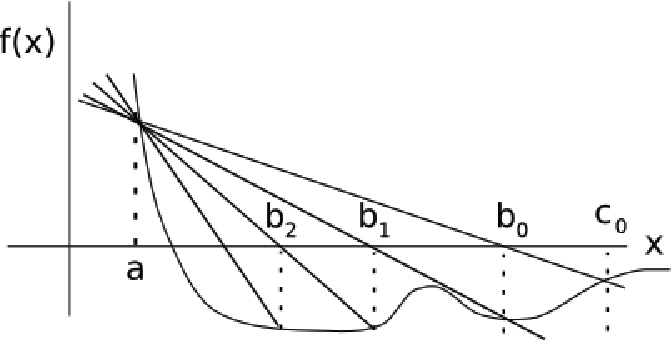
\includegraphics[scale=0.8]{capitulos/capitulo1/figuras/posicaofalsa2-eps-converted-to.pdf}
  \caption{A seqüência de aproximações converge para $b$ por um único lado.}
  \label{fig:posicaofalsa2}
\end{figure}

\end{enumerate}

\subsection{Método da Posição Falsa Modificado}

Esse método elimina o problema de ponto estagnado. Cria-se um contador para verificar quantas vezes o ponto permaneceu um ponto de extremidade. Se o ponto permanecer ponto extremo por mais de duas vezes, divide-se o valor de $f$ (estagnado) por dois.

\begin{figure}[htb]
  %\index{figura da posição falsa modificado}%
  \setlength{\abovecaptionskip}{20pt}
  %%% o valor default de \abovecaptionskip definido para a classe
  %%% article e de 10pt.
  \centering
  %%% VIDE ABAIXO COMENTARIO SOBRE USO DE DIRETORIOS NO PATHNAME
  %%% DOS ARQUIVOS INCLUIDOS.
  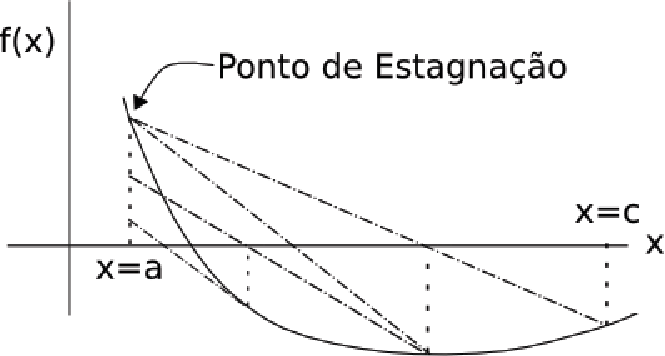
\includegraphics[scale=0.8]{capitulos/capitulo1/figuras/posicaofalsamodificado1-eps-converted-to.pdf}
  \caption{Eliminando o problema do ponto de estagnação.}
  \label{fig:posicaofalsamodificado1}
\end{figure}

\begin{example}
 Usando o método da posição falsa, encontre a menor raíz positiva de $f(x) = \tan(x) - x - 0.5 = 0$, com $\xi = 0.00001$. Sabendo-se que ela se encontra em $ 0.1 < x < 1.4$.

\begin{table}[htp]
\footnotesize
	\centering
		
		\begin{tabular}{|c|c|c|c|c|c|c|}
		\hline		
		\textbf{Iteração} & \textbf{a} & \textbf{b} & \textbf{c} & \textbf{f(a)} & \textbf{f(b)} & \textbf{f(c)}\\
		\hline \hline 
		0 & 0.01 & 0.24771 & 1.4 & -0.49967 & -0.49481 & 3.8979\\
		\hline 
		1 & 0.24771 & 0.48102 & 1.4 & -0.49481 & -0.45911 & 1.9489\\
		\hline 
		2 & 0.48102 & 0.77533 & 1.4 & -0.45911 & -0.29527 & 0.97447\\
		\hline 
		3 & 0.77533 & 1.0110 & 1.4 & -0.29527 & 0.084850 & 0.48724\\
		\hline 
		4 & 0.77533 & 0.95842 & 1.0110 & -0.29527 & -0.034845 & 0.084850\\
		\hline 
		5 & 0.95842 & 0.97374 & 1.0110 & -0.034845 & -0.0027664 & 0.084850\\
		\hline  
		6 & 0.97374 & 0.97603 & 1.0110 & -0.0027664 & 0.0021981 & 0.042425\\
		\hline 
		7 & 0.97374 & 0.97501 & 0.97603 & -0.0027664 & -0.0000061 & 0.0021981\\
		\hline
		8 & 0.97501 & 0.97502 & 0.97603 & -0.0000061 & 0.0000000 & 0.0021981\\
		\hline
		\end{tabular}
	%\caption{Iterações do método da bisseção}
	\caption{Exemplo de iterações do método da posição falsa modificado.}
	\label{tab:posicaofalsamodificado}
\end{table}

$\xi_{_{MAX}} = 0.97603 - 0.97502 = 0.00101$

$\xi = 0.97502 - 0.97501 = 0.00001$

\end{example}